\documentclass{article}
%book , report, letter , beamer
%\usepackage{} 
\usepackage[spanish]{babel}%paquete principal1
\usepackage[utf8]{inputenc}%paquete principal2
\usepackage[T1]{fontenc}%paquete principal3
\usepackage[pdftex]{graphicx}
\usepackage{hyperref}
\usepackage[left=1in, right=1in, top=1in, bottom=1in]{geometry}

\title{Clase de Latex}
\author{Alvaro Chirino\footnote{Comentarios mandar a ...}  }
\date{Abril, 2020}
\begin{document}
\maketitle

\begin{abstract}
kdjfndsjhfbsdjkcbdsjvs dsg
dsgsdgsgs
gdsgsdgsdgg\\

gsdgsdgsdgds
gdsgsdgsd
\end{abstract}

\newpage

\tableofcontents
\listoftables
\listoffigures

\newpage

\section{Introducción}

En el cuadro \ref{tab1} se presenta un ejemplo de tablas

\subsection{Objetivos Generales}

Este documento es introductoria a Latex

\begin{equation}
\frac{1}{x}=y+15+z
\label{eq2}
\end{equation}

\subsection{Objetivos Secundarios}
Los objetivos secundarios son:

\begin{itemize}
\item Ob1 nskjnvs
\item ob2 cdncksjdnvs
\item ob3 cancsjd
\end{itemize}

\begin{enumerate}
\item cdsdv
	\begin{enumerate}
	\item cdsdv
	\item fdsfsdfs
	\item vsdvsd
	\end{enumerate}
\item fdsfsdfs
\item vsdvsd
\end{enumerate}

\section{Motivación}

\textbf{Hola este es mi primer documento en latex en el año 2020}

\section{ecuaciones en Latex}
En esta linea se muestra una sumatoria $\sum_{i=1}$

\begin{equation}
\frac{1}{x}=y+13
\label{eq1}
\end{equation}

En la ecuación \ref{eq1}  se describe ...

\begin{table}[!htb]
\caption{edades por persona}
\centering
\begin{tabular}{|l|l|}
\hline
\textbf{Nombre} & \textbf{Edad} \\ \hline
\hline
\hline
\textbf{Juan}            & 12            \\ \hline
Maria           & 13            \\ \hline
\textbf{Marcos}          & 23            \\ \hline
\textit{Julia}           & 41            \\ \hline
\end{tabular}
\label{tab1}
\end{table}

\begin{figure}[!htp]
\caption{Ejemplo de figura}
\centering
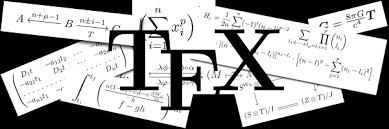
\includegraphics[scale=0.7]{p1}
\label{f1}
\end{figure}


\end{document}
